%%%%%%%%%%%%%%%%% PREAMBLE %%%%%%%%%%%%%%%%%%%%%%%%%%%%
%Change the font size of your document - 10pt, 12.1pt, etc.
\documentclass[letterpaper,11pt,oneside]{article}
\usepackage[T1]{fontenc}
\usepackage[utf8]{inputenc}
\usepackage{setspace}
\usepackage{hyperref}
\usepackage{fontspec}
% \setmainfont[Ligatures=TeX, Numbers={OldStyle}]{Linux Libertine}
% \setmainfont[Ligatures=TeX, Numbers={OldStyle}]{IM FELL DW Pica SC}
% \setmainfont[Ligatures=TeX, Numbers={OldStyle}]{Helvetica Neue Light}
% \setmainfont[Ligatures=TeX, Numbers={OldStyle}]{Avenir}

\usepackage{graphicx}
\graphicspath{ {images/}} %upload your signature to this file
%Change the margins to fit your CV/resume content
\usepackage[left=1in, right=2in, bottom=1.25in, top=1.25in]{geometry}

%Skype information - include your Skype name for a link to add you on Skype
\newcommand*{\Skype}{\href{skype name:mathewin?add}{mathewin}} 
\newcommand{\Absender}[1][\normalsize]{\Skype} 


%Changes the page numbers - {arabic}=arabic numerals, {gobble}=no page numbers, {roman}=Roman numerals
\pagenumbering{gobble}

%%%%%%%%%%%%%%%%% END OF PREAMBLE %%%%%%%%%%%%%%%%%%%%%

\begin{document}

%%%%%%%%%%%%%%%%% NAME OF APPLICANT %%%%%%%%%%%%%%%%%%%

\noindent  \LARGE{\textbf{Mateusz Krzysztof Łącki}}  \\
% \vspace{-2ex}
\normalsize

%%%%%%%%%%%%%%%%% CONTACT INFORMATION %%%%%%%%%%%%%%%%%
% Your email address, website, and Skype name are links to send email, open your website and add you on Skype. 

\begin{minipage}{.1\textwidth}
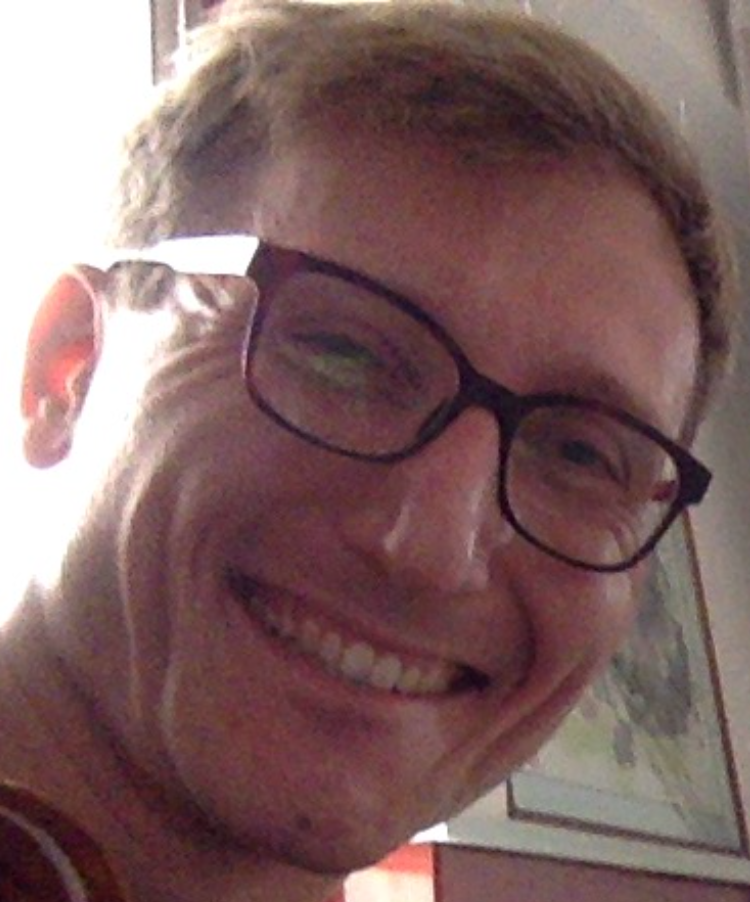
\includegraphics[width=\linewidth]{photo.png}
\end{minipage}
\begin{minipage}{.9\textwidth}
\begin{center}
\begin{tabular}{l l}
 University of Warsaw& \hspace{1in}\href{mailto:matteo.lacki@gmail.com}{matteo.lacki@gmail.com}\\
 Faculty of Mathematics, Informatics,     & \hspace{1in}\href{https://github.com/MatteoLacki}{GitHub: MatteoLacki}   \\
 and Mechanics. & \hspace{1in}Skype: \Absender  \\
 Banacha 2, 02-097 Warszawa, Poland & \hspace{1in}\href{callto:+48 602 39 50 10}{Phone: +48 602 39 50 10}\\
\end{tabular}
\end{center}
\end{minipage}

\vspace{2em}

%%%%%%%%%%%%%%%%% MAIN BODY %%%%%%%%%%%%%%%%%%%%%%%%%%%
% The main body is contained in a tabular environment. To move sections onto the next page, simply end the tabular environment and begin a new tabular environment.

\noindent \begin{tabular}{@{} l l}
 \Large{Education}    & \textbf{University of Warsaw} \\
    & Ph.D., Informatics, awaiting dissertation reviews.\\
    & Fields: Statistics, Computational Proteomics, Applied Mathematics\\
    & Mathematics, M.A. (2013) B.A. (2011).\\
    & \\
    & \textbf{Warsaw School of Economics} \\
    & Quantitative Methods in Economics and Information Systems,\\
    & M.A. (2012), B.A. (2009)\\
    & \\
\Large{Dissertation}&``Computational and Statistical Methods for Mass Spectrometry Data Analysis" \\
    & \\
\Large{Publications}
    & \parbox{5.0in}{\href{http://www.plantphysiol.org/content/early/2017/10/10/pp.17.00904}{L.W. Bielczyński, M.K. Łącki, I. Hoefnagels, A. Gambin, R. Croce, \textit{Leaf and plant age affects photosynthetic performance and photoprotective capacity}, Plant Physiology (2017).}}\\
    & \\
    & \parbox{5.0in}{\href{http://online.liebertpub.com/doi/10.1089/cmb.2017.0156}{M.A. Ciach, M.K. Łącki, B. Miasojedow, F. Lermyte, D. Valkenborg, F. Sobott, A. Gambin, \textit{Estimation of Rates of Reactions Triggered by Electron Transfer in Top Down Mass Spectrometry}, ISBRA Springer LNBI proceedings (2017), extended in the Journal of Computational Biology (2017).}}\\
    & \\
    & \parbox{5.0in}{\href{http://pubs.acs.org/doi/abs/10.1021/acs.analchem.6b01459}{M.K. Łącki, M. Startek, D. Valkenborg, A. Gambin, \textit{IsoSpec: Hyperfast Fine Structure Calculator}, Analytical Chemistry (2017).}}\\
    & \\
    & \parbox{5.0in}{\href{https://link.springer.com/article/10.1007/s13361-016-1444-7}{F. Lermyte, M.K. Łącki, Dirk Valkenborg, Anna Gambin, Frank Sobott, \textit{Conformational space and stability of ETD charge reduction products of ubiquitin}, Journal of the American Society for Mass Spectrometry (2017).}}\\
    & \\
    & \parbox{5.0in}{\href{https://link.springer.com/article/10.1007/s11222-015-9579-0}{M.K. Łącki, B. Miasojedow, \textit{State dependent swap strategies and automatic reduction of number of temperatures in adaptive parallel tempering algorithm}, Statistics and Computing (2016).}}\\
    & \\
    & \parbox{5.0in}{\href{http://www.sciencedirect.com/science/article/pii/S1387380615002572}{F. Lermyte, M.K. Łącki, D. Valkenborg, A. Gambin, F. Sobott, \textit{Understanding reaction pathways in top-down ETD by dissecting isotope distributions: a mammoth task}, International Journal of Mass Spectrometry (2015).}}\\
    & \\
\Large{Preprints}
    & \parbox{5.0in}{\href{https://arxiv.org/abs/1708.00234}{M.K. Łącki, F. Lermyte, B. Miasojedow, M. Startek, F. Sobott, D. Valkenborg, A. Gambin, \textit{MassTodon: A tool for modelling electron transfer reactions in top-down mass spectrometry}}.}\\
    & \href{masstodonpy.readthedocs.io/}{Online documentation}. \href{https://github.com/MatteoLacki/MassTodonPy}{Source code}.\\
\end{tabular}
\begin{tabular}{@{} l l}
\Large{Grants}
    & \parbox{5.0in}{NCN: No. 2015/17/N/ST6/03565 - leader of grant \textit{Modelling of fragmentation of biomolecules induced by electron transfer in mass spectrometry}.}\\
    &\\
\Large{Awards}
    & \parbox{5.0in}{Stipend for the best PhD student of the Faculty of Mathematics, Informatics, and Mechanics of the University of Warsaw in 2017}\\
    &\\
\Large{Workshops}
    & \parbox{5.0in}{de.NBI, \textit{From Big Data to Big Insights}, Dagstuhl, September 2016\\
      EMBO Computational Biology Workshop, Goniądz, February 2015\\
      4th International Proteome Discoverer Users’ Meeting, Bremen 2015\\
      1st International Mass Spectrometry School, Siena 2013}\\
    &\\    
\Large{Organized} 
    & EMBO Computational Biology Workshop 2, April 2016, Jabłonna, Poland\\
\Large{Conferences}
    & RECOMB-seq 2015, Warsaw, Poland\\
    &\\
\Large{Internships}
    & \parbox{5.0in}{Antwerp, Centre for Proteomics, November 2014 — February 2015.\\
    ARUP Laboratories, 23 June — 11 July 2014, Salt-Lake City, Utah, USA,\\
    \quad visiting prof. Alan L. Rockwood.\\
    Antwerp, Centre for Proteomics, February 2014}\\
    &\\
  \Large{Teaching}  
    & \parbox{5.0in}{Advanced Monte Carlo Methods, Introduction to Statistics, Stochastic Simulations, Statistics II, Ordinary Differential Equations, Computational Molecular Medicine.}\\
    &\\
% \Large{Awards and }    & \textbf{Graduate Student Teacher of the Year, Department} \\
%  \Large{Fellowships}   & Course Name, 2014-2015 \\
%     & \\
%     & \textbf{Fulbright Scholarship} \\
%     & City, Country, 2006-2009 \\
%     & \\
  \Large{Languages}   & Polish (native), English (proficient), French (advanced), Italian (advanced), \\
\Large{and Skills}    & Python developper, C/C++, R, \LaTeX.\\
\end{tabular}

\vspace{12ex}
%%%%%%%%%%%%%%%%% REFERENCES %%%%%%%%%%%%%%%%%%%%%%%%%%
% The reference section has links to your references' websites and email addresses.

\noindent \begin{tabular}{@{} l l l}
 \Large{References} & \href{https://www.mimuw.edu.pl/~aniag/}{Prof. Anna Gambin} & \href{https://www.elixir-belgium.org/organisation/collaborators/dirkvalkenborg}{Dr Dirk Valkenborg} \\
 & Faculty of Mathematics, Informatics,&  Centre for Statistics,\\
 & and  Mechanics, University of Warsaw &  University of Hasselt \\
 & \small{\href{mailto:aniag@mimuw.edu.pl}{aniag@mimuw.edu.pl},+1\,(123)\,456-7899} & \small{\href{dirk.valkenborg@uhasselt.be}{dirk.valkenborg@uhasselt.be},+32\,(0)\,11 26 82 43} \\
&& \\
 & \href{https://scholar.google.pl/citations?user=_PedoD8AAAAJ&hl=en}{Dr Błażej Miasojedow} & \href{https://www.uantwerpen.be/en/rg/bams/people/prof--dr--frank-sobo/}{Prof. Dr Frank Sobott}  \\
 & Faculty of Mathematics, Informatics, &  Astbury Centre for Structural Molecular Biology\\
 & and  Mechanics, University of Warsaw &  University of Leeds \\
 & \small{\href{bmiasojedow@gmail.com}{bmiasojedow@gmail.com},+48\,22\,55 44 441} & \small{\href{mailto:f.sobott@leeds.ac.uk}{f.sobott@leeds.ac.uk},\,0\,113\,343\,2576} \\
\end{tabular}



% \clearpage
% \setlength\parindent{0cm}
% \pagenumbering{gobble} %cover letter should be one page, {gobble}=no page number



% \begin{flushright}
%  \today                           \\
%  \vspace{1em}                              
%  Home University            \\
%  Home Department                  \\
%  Street Address                       \\
%  City, State. 12345-67899   \\
%  Phone: +1 (123) 456-7899         \\
% \href{mailto:john.smith@email.com}{john.smith@email.com}  \\ %insert your email address here for a clickable link
% \end{flushright}


% \begin{flushleft}
%  \textbf{Faculty Search Committee}         \\
%  Name of University \\
% Name of Department                  \\
% Address of Department \\
% City, State. Zip Code
% \end{flushleft}

% \vspace{2em}

% Dear Sir or Madam, \\

% \vspace{1em}
% \onehalfspacing

% My name is John Smith and I'm applying to the academic position in this subject at the Name of University. I have experience teaching something and something else and my research focuses on this and that. I completed my Ph.D. in this subject in September 2015 at my alma mater.

% \vspace{1em}

% My educational background is in this and that at the former university along with an earned Master's and Ph.D. degree in this recent subject at this alma mater. I have taught this, that, and everything else. My research is in this area, that area, and another area still.

% \vspace{1em}

% My dissertation advisor, Professor Head Adviser, and committee members Professor Two and Professor Three have been instrumental throughout my time at Home University. Please feel free to contact me with any questions.

% \vspace{1em}

% \begin{flushright}
% Sincerely, \\
% \vspace{1em} 
% \includegraphics[scale=0.4]{Phillips} \\ %insert your own signature here
% \vspace{1em} 
% John Smith \\
% \end{flushright}

\end{document}

